\documentclass[12pt,a4paper]{article}
\usepackage[UTF8]{ctex}                    % 中文支持
\usepackage{geometry}                      % 页面布局
\usepackage{amsmath,amssymb,amsthm}        % 数学符号与定理
\usepackage{mathtools,bm}                  % 高级数学工具
\usepackage{graphicx}                      % 图片插入
\usepackage{hyperref}                      % 超链接
\usepackage{tikz}
\hypersetup{
	pdfborder = {0 0 0}  % 关闭链接边框
}
\usepackage{cleveref}
\usepackage{booktabs}                      % 三线表
\usepackage[numbers,sort&compress]{natbib} % 参考文献
\usepackage{caption}                       % 图表标题
\usepackage[shortlabels]{enumitem}         % 列表环境

% ========== 页面布局 ==========
\geometry{left=2.5cm, right=2.5cm, top=2.5cm, bottom=2.5cm}
\setlength{\parskip}{0.5em}                % 段落间距
\renewcommand{\baselinestretch}{1.2}       % 行距

% ========== 数学命令 ==========
\newcommand{\diff}{\mathop{}\!\mathrm{d}}  % 微分符号
\newcommand{\R}{\mathbb{R}}                % 实数集
\newcommand{\C}{\mathbb{C}}                % 复数集
\newcommand{\Z}{\mathbb{Z}}                % 整数集
\newcommand{\Lspace}{L^2(-l,l)}            % L²空间

% ========== 定理环境 ==========
% 定义题目环境
\newtheorem{problem}{题}
% 定义解题环境
\newtheorem*{solution}{解}

\newtheorem{example}{例题}

\newtheorem{corollary}{推论}

\newtheorem{proposition}{命题}

\newtheorem{lemma}{引理}

% ========== 文档信息 ==========


\vspace{1cm}



%\title{偏微分方程第三次作业}
%\author{22数学1陈柏均202225110102}
%\date{\today}


\begin{document}
	
	\begin{center}
		\LARGE 偏微分方程第三次作业 \\
		\vspace{0.5cm}
		\large 班级:22数学1 \quad 姓名:陈柏均 \quad 学号:202225110102
	\end{center}
	
	%\maketitle




\begin{problem}
	求解方程
	\[
	\begin{cases}
		u_{tt} - u_{xx} = t\sin x, & -\infty < x < +\infty, \quad t > 0 \\
		u|_{t=0} = 0, \quad u_t|_{t=0} = \sin x, & -\infty < x < +\infty.
	\end{cases}
	\]
	(提示:齐次化原理+达朗贝尔公式)
	
\end{problem}

\begin{solution}
步骤1.齐次方程求解
	
	\noindent
	齐次波动方程\eqref{eq:5}的初值问题为:
	\begin{equation}\label{eq:5}
		\begin{cases}
			u_{tt} - u_{xx} = 0, & -\infty < x < +\infty, \quad t > 0 \\
			u|_{t=0} = 0, \quad u_t|_{t=0} = \sin x, & -\infty < x < +\infty.
		\end{cases}
	\end{equation}
	应用达朗贝尔公式,解为:
	\[
	u_h(x, t) = \frac{1}{2} \int_{x - t}^{x + t} \sin s \, ds
	\]
	计算积分:
	\[
	\int_{x - t}^{x + t} \sin s \, ds = -\cos s \Big|_{x - t}^{x + t} = -\cos(x + t) + \cos(x - t)
	\]
	利用三角恒等式展开:
	\[
	\cos(x + t) = \cos x \cos t - \sin x \sin t \\
	\cos(x - t) = \cos x \cos t + \sin x \sin t
	\]
	代入后得到:
	\[
	u_h(x, t) = \frac{1}{2} \left[ (\cos x \cos t + \sin x \sin t) - (\cos x \cos t - \sin x \sin t) \right] = \sin x \sin t
	\]
	
	步骤2. 非齐次方程求解
	
	\noindent
	非齐次方程\eqref{eq:6}的初值问题为:
	\begin{equation}\label{eq:6}
		\begin{cases}
			u_{tt} - u_{xx} = t \sin x, & -\infty < x < +\infty, \quad t > 0 \\
			u|_{t=0} = 0, \quad u_t|_{t=0} = 0, & -\infty < x < +\infty.
		\end{cases}
	\end{equation}
	应用齐次化原理,非齐次解为:
	\[
	u_p(x, t) = \int_0^t \frac{1}{2} \int_{x - (t - \tau)}^{x + (t - \tau)} \tau \sin s \, ds \, d\tau
	\]
	计算内部积分:
	\[
	\int_{x - (t - \tau)}^{x + (t - \tau)} \tau \sin s \, ds = \tau \left[ -\cos(x + t - \tau) + \cos(x - t + \tau) \right]
	\]
	利用三角恒等式:
	\[
	\cos(x - t + \tau) - \cos(x + t - \tau) = 2 \sin x \sin(t - \tau)
	\]
	代入后得到:
	\[
	u_p(x, t) = \sin x \int_0^t \tau \sin(t - \tau) \, d\tau
	\]
	变量替换 \(u = t - \tau\),计算积分:
	\[
	\int_0^t \tau \sin(t - \tau) \, d\tau = t - \sin t
	\]
	因此,非齐次解为:
	\[
	u_p(x, t) = \sin x (t - \sin t)
	\]
	
	步骤3.总解求解
	
	\noindent
	将齐次解和非齐次解相加,得到总解:
	\[
	u(x, t) = u_h(x, t) + u_p(x, t) = \sin x \sin t + \sin x (t - \sin t) = t \sin x
	\]
	
	
\end{solution}



\newpage
% ========================= 第2题 =========================
\begin{problem}
	解下列半直线上的混合问题
	\[
	\begin{cases}
		u_{tt} - a^2 u_{xx} = 0, & x > 0, \quad t > 0 \\
		u|_{t=0} = 2x, & u_t |_{t=0} = x^2, \\
		u|_{x=0} = 0, & t \geq 0.
	\end{cases}
	\]
\end{problem}


	
	\begin{solution}
		
	步骤1. 奇延拓处理
			
		\noindent
		定义延拓函数以处理半无界边界条件:
		\[
		\overline{u}(x,t) = 
		\begin{cases} 
			u(x,t) & x \geq 0 \\
			-u(-x,t) & x < 0 
		\end{cases}, \quad
		\overline{h}(x) = 
		\begin{cases} 
			x^2 & x \geq 0 \\
			-(-x)^2 = -x^2 & x < 0 
		\end{cases}
		\]
		边界条件满足:
		\[
		\overline{g}(0) = 0, \quad \overline{h}(0) = 0
		\]
		
		步骤2. 达朗贝尔公式应用
			
		\noindent
		扩展后的问题解为:
		\[
		\overline{u}(x,t) = \frac{1}{2}\left[\overline{g}(x+at) + \overline{g}(x-at)\right] + \frac{1}{2a}\int_{x-at}^{x+at} \overline{h}(y) \, dy
		\]
		其中 \(\overline{g}(x) = 2x\)。
		
		步骤3. 分区域求解
	
		\noindent
	情形一:\(x \geq at\)(远离边界)
		
		\noindent
		积分区间完全在正半轴:
		\[
		\begin{aligned}
			\overline{u}(x,t) 
			&= \frac{1}{2}[2(x+at) + 2(x-at)] + \frac{1}{2a}\int_{x-at}^{x+at} y^2 \, dy \\
			&= 2x + \frac{1}{6a}\left[(x+at)^3 - (x-at)^3\right] \\
			&= 2x + \frac{t}{3}\left[3x^2 + a^2t^2\right] \\
			&= 2x + tx^2 + \frac{1}{3}a^2t^3
		\end{aligned}
		\]
		
			
		\noindent
		情形二:\(0 < x < at\)(近边界)
		
		积分区间跨越原点,需考虑奇延拓:
		\[
		\begin{aligned}
			\overline{u}(x,t) 
			&= \frac{1}{2}[2(x+at) - 2(at-x)] + \frac{1}{2a}\int_{at-x}^{x+at} y^2 \, dy \\
			&= 2x + \frac{1}{6a}\left[(x+at)^3 - (at-x)^3\right] \\
			&= 2x + \frac{x}{3a}\left[x^2 + 3a^2t^2\right] \\
			&= \frac{1}{3a}x^3 + (at^2 + 2)x
		\end{aligned}
		\]
		
	步骤4. 综合解
			
		\noindent
		最终解为分段函数:
		\[
		u(x,t) = 
		\begin{cases}
			2x + tx^2 + \dfrac{1}{3}a^2t^3 & x \geq at \\
			\dfrac{1}{3a}x^3 + (at^2  + 2)x & 0 < x < at
		\end{cases}
		\]
	\end{solution}








\newpage
% ========================= 第3题 =========================
\begin{problem}
	求下列特征值问题的特征值和特征函数
	\[
	\begin{cases}
		X''(x) + \lambda X(x) = 0, & 0 < x < l, \\
		X(0) = X'(l) = 0.
	\end{cases}
	\]
\end{problem}

\begin{solution}
	步骤1. 当 \(\lambda < 0\) 时
		
	\noindent
	设 \(\lambda = -\mu^2\ (\mu > 0)\),方程通解为:
	\[
	X(x) = C_1 \cosh(\mu x) + C_2 \sinh(\mu x)
	\]
	代入边界条件 \(X(0)=0\):
	\[
	C_1 \cosh(0) + C_2 \sinh(0) = 0 \implies C_1 = 0
	\]
	导数表达式:
	\[
	X'(x) = \mu C_2 \cosh(\mu x)
	\]
	代入 \(X'(l)=0\):
	\[
	\mu C_2 \cosh(\mu l) = 0 \implies C_2 = 0
	\]
	故仅有零解,排除负特征值。
	
	步骤2. 当 \(\lambda = 0\) 时
		
	\noindent
	方程简化为:
	\[
	X''(x) = 0 \implies X(x) = C_1 x + C_2
	\]
	代入边界条件:
	\[
	X(0) = C_2 = 0,\quad X'(l) = C_1 = 0
	\]
	同样仅有零解,排除零特征值。
	
	步骤3. 当 \(\lambda > 0\) 时
		
	\noindent
	设 \(\lambda = \mu^2\ (\mu > 0)\),方程通解为:
	\[
	X(x) = A \cos(\mu x) + B \sin(\mu x)
	\]
	代入 \(X(0)=0\):
	\[
	A \cos(0) + B \sin(0) = 0 \implies A = 0
	\]
	导数表达式:
	\[
	X'(x) = \mu B \cos(\mu x)
	\]
	代入 \(X'(l)=0\):
	\[
	\mu B \cos(\mu l) = 0
	\]
	要求非零解,需满足:
	\[
	\cos(\mu l) = 0 \implies \mu l = \frac{(2n+1)\pi}{2},\ n=0,1,2,\cdots
	\]
	得特征值:
	\[
	\lambda_n = \left( \frac{(2n+1)\pi}{2l} \right)^2
	\]
	对应特征函数:
	\[
	X_n(x) = B_n \sin\left( \frac{(2n+1)\pi}{2l} x \right)
	\]
	
	

\end{solution}



\newpage
% ========================= 第4题 =========================
\begin{problem}
	求弦振动方程
	\[
	u_{tt} - a^2 u_{xx} = 0, \quad 0 < x < l, \quad t > 0
	\]
	满足以下定解条件的解
	\[
	\begin{cases}
		u|_{t=0} = \sin \dfrac{3\pi x}{2l}, & u_t |_{t=0} = \sin \dfrac{5\pi x}{2l}, \quad 0 \leq x \leq l, \\
		u|_{x=0} = u_x |_{x=l} = 0, & t \geq 0.
	\end{cases}
	\]
\end{problem}

	
\begin{solution}
	\textbf{方法1.分离变量法}
	
	步骤1. 分离变量
		
	\noindent
	设解为 \( u(x,t) = X(x)T(t) \),代入方程得:
	\[
	\frac{T''}{a^2 T} = \frac{X''}{X} = -\lambda
	\]
	分离为两个常微分方程:
	\[
	\begin{cases}
		X'' + \lambda X = 0 \\
		T'' + a^2 \lambda T = 0
	\end{cases}
	\]
	
	步骤2. 求解空间方程
		
	\noindent
	边界条件 \( X(0) = X'(l) = 0 \),分三种情况讨论:
		
	\noindent
	情形1. \(\lambda < 0\)
		
	\noindent
	设 \(\lambda = -\mu^2\ (\mu > 0)\),通解为:
	\[
	X(x) = C_1 \cosh(\mu x) + C_2 \sinh(\mu x)
	\]
	代入边界条件 \( X(0) = 0 \) 得 \( C_1 = 0 \)。再代入 \( X'(l) = 0 \):
	\[
	\mu C_2 \cosh(\mu l) = 0 \implies C_2 = 0
	\]
	无非零解,排除负特征值。
		
	\noindent
	情形2. \(\lambda = 0\)
		
	\noindent
	通解为:
	\[
	X(x) = C_1 x + C_2
	\]
	代入边界条件得 \( C_1 = C_2 = 0 \),排除零特征值。
		
	\noindent
	情形3. \(\lambda > 0\)
		
	\noindent
	设 \(\lambda = \mu^2\ (\mu > 0)\),通解为:
	\[
	X(x) = A \cos(\mu x) + B \sin(\mu x)
	\]
	代入 \( X(0) = 0 \) 得 \( A = 0 \)。再代入 \( X'(l) = 0 \):
	\[
	\mu B \cos(\mu l) = 0 \implies \cos(\mu l) = 0
	\]
	解得特征值:
	\[
	\mu l = \frac{(2n+1)\pi}{2} \implies \lambda_n = \left( \frac{(2n+1)\pi}{2l} \right)^2,\quad n=0,1,2,\cdots
	\]
	对应特征函数:
	\[
	X_n(x) = B_n\sin\left( \frac{(2n+1)\pi}{2l} x \right)
	\]
	
	步骤3. 求解时间方程
		
	\noindent
	对应每个 \(\lambda_n\),时间方程为:
	\[
	T_n'' + a^2 \lambda_n T_n = 0
	\]
	通解为:
	\[
	T_n(t) = C_n \cos\left( \frac{(2n+1)\pi a}{2l} t \right) + D_n \sin\left( \frac{(2n+1)\pi a}{2l} t \right)
	\]
	
	步骤4. 合成通解
		
	\noindent
	由叠加原理可得($B_n$被吸收了):
	\[
	u(x,t) = \sum_{n=0}^\infty \sin\left( \frac{(2n+1)\pi}{2l} x \right) \left[ C_n \cos\left( \frac{(2n+1)\pi a}{2l} t \right) + D_n \sin\left( \frac{(2n+1)\pi a}{2l} t \right) \right]
	\]
	
步骤5. 确定系数得解
		
	\noindent
	代入初始条件 \( u(x,0) = \sin\frac{3\pi x}{2l} \):
	\[
	\sum_{n=0}^\infty C_n \sin\left( \frac{(2n+1)\pi}{2l} x \right) = \sin\frac{3\pi x}{2l}
	\]
	比较系数得:
	\[
	C_1 = 1,\quad C_n = 0\ (n \neq 1)
	\]
	
	代入初始条件 \( u_t(x,0) = \sin\frac{5\pi x}{2l} \):
	\[
	\sum_{n=0}^\infty D_n \frac{(2n+1)\pi a}{2l} \sin\left( \frac{(2n+1)\pi}{2l} x \right) = \sin\frac{5\pi x}{2l}
	\]
	比较系数得:
	\[
	D_2 = \frac{2l}{5\pi a},\quad D_n = 0\ (n \neq 2)
	\]
	
	\[
	u(x,t) = \sin\frac{3\pi x}{2l} \cos\left( \frac{3\pi a}{2l} t \right) + \frac{2l}{5\pi a} \sin\frac{5\pi x}{2l} \sin\left( \frac{5\pi a}{2l} t \right)
	\]
	
	
	\newpage
	\textbf{方法2.反射法达朗贝尔公式做延拓}


考虑初边值问题
\begin{equation*}
	\begin{cases}
		u_{tt} - a^2 u_{xx} = 0, & 0 < x < L, \ t > 0, \\
		u(x, 0) = f(x), \ u_t(x, 0) = g(x), & 0 \leq x \leq L, \\
		u(0, t) = 0, \ u_x(L, t) = 0, & t \geq 0.
	\end{cases}
\end{equation*}
	
	有时可以用达朗贝尔公式求解初边值问题。又设 \(f, g \in C^2\),且满足相容条件:
\begin{equation}
	\begin{aligned}
		f(0) & = 0, & f'(L)  = 0, \\
		g(0) & =0, & g'(L)  = 0,
	\end{aligned}
\end{equation}
	奇延拓 ($x=0$) $+$ 偶延拓 ($x=L$),周期$4L$                                                                                                                                                                                                                                                                                                                                                                                                                                                                                                                                                                                                                                                                                                                                                                                                                                                                                                                                                                                                                                                                                                                                                                                                                                                                                                                                                                                                                                                                                                                                                                                                                                                                                                                                                                                                                                                                                                                                                                                                                                                                                                                                                                                                                                                                                                                                                                                                                                                                                                                                                                                                                                                                                                                                                                                                                                                                                                                                                                                                                                                                                                                                                                                                                                                                                                                                                                                                                                                                                                                                                                                                                                                                                                                                                                                                                                                                                                                                                                                                                                                                                                                                                                                                                                                                                                                                                                                                                                                                                                                                                                                                                                                                                                                                                                                                                                                                                                                                                                                                                                                                                                                                                                                                                                                                                                                                                                                                                                                                                                                                                                                                                                                                                                                                                                                                                                                                                                                                                                                                                                                                                                                                                                                                                                                                                                                                                                                                                                                                                                                                                                                                                                                                                                                                                                                                                                                                                                                                                                                                                                                                                                                                                                                                                                                                                                                                                                                                                                                                                                                                                                                                                                                                                                                                                                                                                                                                                                                                                                                                                                                                                                                                                                                                                                                                                                                                                                                                                                                                                                                                                                                                                                                                                                                                                                                                                                                                                                                                                                                                                                                                                                                                                                                                                                                                                                                                                                                                                                                                                                                                                                                                                                                                                                                                                                                                                                                                                                                                                                                                                                                                                                                                                                                                                                                                                                                                                                                                                                                                                                                                                                                                                                                                                                                                                                                                                                                                                                                                                                                                                                                                                                                                                                                                                                                                                                                                                                                                                                                                                                                                                                                                                                                                                                                                                                                                                                                                                                                                                                                                                                                                                                                                                                                                                                                                                                                                                                                                                                                                                                                                                                                                                                                                                                                                                                                                                                                                                                                                                                                                                                                                                                                                                                                                                                                                                                                                                                                                                                                                                                                                                                                                                                                                                                                                                                                                                                                                                                                                                                                                                                                                                                                                                                                                                                                                                                                                                                                                                                                                                                                                                                                                                                                                                                                                                                                                                                                                                                                                                                                                                                                                                                                                                                                                                                                                                                                                                                                                                                                                                                                                                                                                                                                                                                                                                                                                                                                                                                                                                                                                                                                                                                                                                                                                                                                                                                                                                                                                                                                                                                                                                                                                                                                                                                                                                                                                                                                                                                                                                                                                                                                                                                                                                                                                                                                                                                                                                                                                                                                                                                                                                                                                                                                                                                                                                                                                                                                                                                                                                                                                                                                                                                                                                                                                                                                                                                                                                                                                                                         .

	题目中的$f$,$g$延拓之后还是原函数。
	\begin{equation*}
		= \frac{1}{2} \left[ \sin\left( \frac{3\pi}{2l}(x + at) \right) + \sin\left( \frac{3\pi}{2l}(x - at) \right) \right]	+ \frac{1}{2a} \int_{x - at}^{x + at} \sin\left( \frac{5\pi}{2l} y \right) dy
	\end{equation*}
	


计算第一项:

由于 $\quad \sin(A + B) + \sin(A - B) = 2 \sin A \cos B$

	
	\begin{equation*}
		\therefore \sin\left( \frac{3\pi}{2l}(x + at) \right) = 2 \sin\left( \frac{3\pi}{2l} x \right) \cos\left( \frac{3\pi}{2l} at \right)
	\end{equation*}
	
	计算第二项:
	
	\begin{equation*}
		\int_{x - at}^{x + at} \sin\left( \frac{5\pi}{2l} y \right) dy	= \left. -\frac{2l}{5\pi} \cos\left( \frac{5\pi}{2l} y \right) \right|_{x - at}^{x + at}
	\end{equation*}
	
	\begin{equation*}
		= -\frac{2l}{5\pi} \left[ \cos\left( \frac{5\pi}{2l}(x + at) \right) - \cos\left( \frac{5\pi}{2l}(x - at) \right) \right]
	\end{equation*}
	



	由于$	\cos(A + B) - \cos(A - B) = -2 \sin A \sin B$

	
	\begin{equation*}
		\int_{x - at}^{x + at} \sin\left( \frac{5\pi}{2l} y \right) dy = -\frac{2l}{5\pi} \cdot (-2) \sin\left( \frac{5\pi}{2l} x \right) \sin\left( \frac{5\pi}{2l} at \right)
	\end{equation*}
	
	\begin{equation*}
		= \frac{4l}{5\pi} \sin\left( \frac{5\pi}{2l} x \right) \sin\left( \frac{5\pi}{2l} at \right)
	\end{equation*}
	
	\begin{equation*}
	 	u(x,t) =\sin\left( \frac{3\pi x}{2l} \right) \cos\left( \frac{3\pi at}{2l} \right) + \frac{2l}{5\pi a} \sin\left( \frac{5\pi x}{2l} \right) \sin\left( \frac{5\pi at}{2l} \right)
	\end{equation*}
	
	
	
	
	
	
\end{solution}




\newpage
% ========================= 第5题 =========================
\begin{problem}
	求解热传导方程
	\[
	u_t - u_{xx} = 0, \quad -\infty < x < \infty, \quad t > 0
	\]
	的Cauchy问题,已知初始条件为
	\begin{enumerate}[label=(\arabic*)]
		\item \( u|_{t=0} = \sin x \);
		\item \( u|_{t=0} = e^{-|x|} \);
		\item \( u|_{t=0} = x^2 + 1 \);
		\item \( u|_{t=0} = x + x^2 \).
	\end{enumerate}
\end{problem}

\begin{solution}

	热传导方程的解由热核卷积给出:
	\[
	u(x,t) = \frac{1}{\sqrt{4\pi t}} \int_{-\infty}^\infty \psi(y) e^{-\frac{(x-y)^2}{4t}} dy
	\]
	公式详细推导在我github上的偏微分笔记上有\href{https://github.com/Albert-Chen04/Partial-differential-equation}{GitHub - Albert-Chen04/Partial-differential-equation}
	
	下面是高斯型函数一些积分的计算
	
	
	
\begin{proposition}
	\label{ex:1}
	实数形式的高斯积分:
	\begin{equation}
		\int_{-\infty}^{+\infty} e^{-a(x-b)^2} dx = \sqrt{\frac{\pi}{a}} \quad (a>0, b \in \mathbb{R})
	\end{equation}
\end{proposition}
	
	\begin{proof}
		\begin{equation*}
		A^2 = \left( \int_{-\infty}^{+\infty} e^{-a(x-b)^2} dx \right) \left( \int_{-\infty}^{+\infty} e^{-a(y-b)^2} dy \right)
	\end{equation*}
	
	\begin{equation*}
		= \int_{-\infty}^{+\infty} \int_{-\infty}^{+\infty} e^{-a((x-b)^2 + (y-b)^2)} dx dy
	\end{equation*}
	
	由极坐标变量替换可得
	
	\begin{equation*}
		(x - b)^2 + (y - b)^2 = r^2
	\end{equation*}
	
	\begin{equation*}
		\begin{cases}
			x - b = r \cos\theta \\
			y - b = r \sin\theta
		\end{cases}
	\end{equation*}
	
	\begin{equation*}
		\begin{cases}
			dx = \cos\theta \, dr - r \sin\theta \, d\theta \\
			dy = \sin\theta \, dr + r \cos\theta \, d\theta
		\end{cases}
	\end{equation*}
	
	\begin{equation*}
		J = \begin{vmatrix}
			\cos\theta & -r \sin\theta \\
			\sin\theta & r \cos\theta
		\end{vmatrix} = r
	\end{equation*}
	
	\begin{equation*}
		dx dy = r \, d\theta \, dr
	\end{equation*}
	
	\begin{equation*}
		A^2 = \int_{-\pi}^{\pi} \int_{0}^{\infty} e^{-ar^2} r \, dr \, d\theta	= \frac{1}{2} \int_{-\pi}^{\pi} \int_{0}^{\infty} e^{-ar^2} d(r^2) \, d\theta
	\end{equation*}
	
	
	\begin{equation*}
		= \frac{1}{2} \int_{-\pi}^{\pi} \left[ -\frac{1}{a} e^{-ar^2} \Big|_{0}^{+\infty} \right] d\theta= \frac{1}{2} \int_{-\pi}^{\pi} \frac{1}{a} \, d\theta	= \frac{\pi}{a}
	\end{equation*}
	
	
	\begin{equation*}
	\therefore	\int_{-\infty}^{+\infty} e^{-a(x-b)^2} dx = \sqrt{\frac{\pi}{a}}
	\end{equation*}
	
	\end{proof}

\begin{corollary}\label{ex:5}
	$\int_{-\infty}^{+\infty} x^2 e^{-a x^2} dz = \frac{1}{2} \pi^{\frac{1}{2}} a^{-\frac{3}{2}}$
\end{corollary}



\begin{proof}
	
	
	\begin{equation*}
		\text{设} \quad \Phi(a) = \int_{-\infty}^{+\infty} e^{-a x^2} dx = \sqrt{\frac{\pi}{a}}
	\end{equation*}
	
	\begin{equation*}
		\frac{d\Phi}{da} = -\int_{-\infty}^{+\infty} x^2 e^{-a x^2} dx = \frac{d}{da} \left( \pi^{\frac{1}{2}} a^{-\frac{1}{2}} \right) = \pi^{\frac{1}{2}} a^{-\frac{3}{2}} \cdot \left( -\frac{1}{2} \right)
	\end{equation*}
	
	\begin{equation*}
		\therefore \int_{-\infty}^{+\infty} x^2 e^{-a x^2} dx = \frac{1}{2} \pi^{\frac{1}{2}} a^{-\frac{3}{2}}
	\end{equation*}
\end{proof}	


\begin{corollary}\label{ex:6}
	$	\int_{-\infty}^{+\infty} (z + bx)^2 e^{-a z^2} dz=	= \frac{1}{2} \pi^{\frac{1}{2}} a^{-\frac{3}{2}} + b^2 x^2 \sqrt{\frac{\pi}{a}}$
\end{corollary}

\begin{proof}
	展开得
	\begin{equation*}
		= \int_{-\infty}^{+\infty} z^2 e^{-a z^2} dz + \int_{-\infty}^{+\infty} 2 z b x e^{-a z^2} dz + b^2 x^2 \int_{-\infty}^{+\infty} e^{-a z^2} dz
	\end{equation*}
	
	\begin{equation*}
		= \frac{1}{2} \pi^{\frac{1}{2}} a^{-\frac{3}{2}} + b^2 x^2 \sqrt{\frac{\pi}{a}}
	\end{equation*}
	
\end{proof}



\begin{proposition}
	\label{ex:2}
	推广复数形式的高斯积分:
	\begin{equation}
		\int_{-\infty}^{+\infty} e^{-a(x-bi)^2} dx = \sqrt{\frac{\pi}{a}} \quad (a>0, b \in \mathbb{R})
	\end{equation}
\end{proposition}

\begin{proof}
	该积分等价于证明 $\int_{-\infty+bi}^{+\infty+bi} e^{-az^2} dz = \sqrt{\frac{\pi}{a}}$。即$\int_{AB} e^{-az^2} dz$, 我们通过围道积分来证明。
	
	考虑复变函数 $f(z) = e^{-az^2}$,它在整个复平面上解析(为整函数)。我们选取如下所示的矩形闭合围道 $C$ 进行积分,该围道由四条路径组成:$AB$, $BC$, $CD$ 和 $DA$。
	
	\begin{center}
		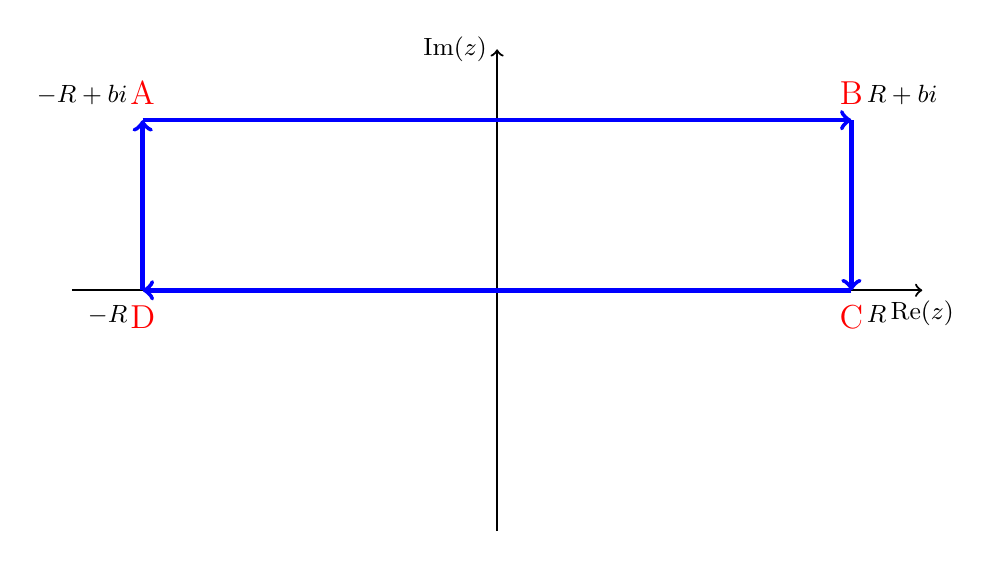
\begin{tikzpicture}[scale=1.8, font=\small]
			% Define coordinates
			\def\R{2.5}
			\def\b{1.2}
			
			% Draw axes
			\draw[->, thick] (-\R-0.5, 0) -- (\R+0.5, 0) node[below] {$\mathrm{Re}(z)$};
			% Adjusted y-axis to not overlap with labels
			\draw[->, thick] (0, -\b-0.5) -- (0, \b+0.5) node[left] {$\mathrm{Im}(z)$};
			
			% Define the vertex coordinates
			\coordinate (D) at (-\R, 0);
			\coordinate (C) at (\R, 0);
			\coordinate (B) at (\R, \b);
			\coordinate (A) at (-\R, \b);
			
			% --- MODIFICATION: Path labels C1, C2 etc. are removed ---
			% Draw paths with arrows only
			\draw[blue, ultra thick, ->] (C) -- (D);
			\draw[blue, ultra thick, ->] (B) -- (C);
			\draw[blue, ultra thick, ->] (A) -- (B);
			\draw[blue, ultra thick, ->] (D) -- (A);
			
			% Add vertex coordinate labels (black)
			\node[below left=2pt] at (D) {$-R$};
			\node[below right=2pt] at (C) {$R$};
			\node[above right=2pt] at (B) {$R+bi$};
			\node[above left=2pt] at (A) {$-R+bi$};
			
			% Add vertex letter labels (red), positioned to avoid overlap
			\node[red, above=2pt, font=\large] at (A) {A};
			\node[red, above=2pt, font=\large] at (B) {B};
			\node[red, below=2pt, font=\large] at (C) {C};
			\node[red, below=2pt, font=\large] at (D) {D};
			
		\end{tikzpicture}
	\end{center}
	
	根据柯西积分定理,函数在闭合围道上的积分为零:
	\begin{equation}\label{kexi}
		\oint_C e^{-az^2} dz = \int_{AB} e^{-az^2} dz + \int_{BC} e^{-az^2} dz + \int_{CD} e^{-az^2} dz + \int_{DA} e^{-az^2} dz = 0
	\end{equation}
	
	我们分别计算 $R \to \infty$ 时各段路径的积分。
	
	
	
	\textbf{1. 路径 $BC$ 与 $DA$:}
	在路径 $BC$ 上,参数化为 $z = R+iy$, $z(b) = R+ib$,$z(0) = R$,$dz=idy$, 其中 $y$ 从 $0$ 到 $b$。
	\begin{equation*}
		\left| \int_{BC} e^{-az^2} dz \right|= \left| \int_{R+bi}^{R} e^{-a(R+iy)^2} i dy \right|= \left| \int_{b}^{0} e^{-a(R+iy)^2} i dy \right| \le \int_{b}^{0} |e^{-a(R^2 - y^2 + 2iRy)}| dy 
	\end{equation*}
	\begin{equation*}
		= \int_{b}^{0} e^{-aR^2} e^{ay^2} dy = e^{-aR^2} \int_{b}^{0} e^{ay^2} dy
	\end{equation*}
	由于 $\int_{b}^{0} e^{ay^2} dy$ 是一个关于 $b$ 的常数,而 $\lim_{R \to \infty} e^{-aR^2} = 0$,所以:
	\begin{equation*}
		\lim_{R \to \infty} \left| \int_{BC} e^{-az^2} dz \right| = 0
	\end{equation*}
	同理可证,路径 $AD$ 的积分也为零。
	
	\textbf{2. 路径 $AB$:}
	在路径 $AB$ 上,参数化为 $z=x+bi$, $dz=dx$, 其中 $x$ 从 $R$ 变化到 $-R$。,由柯西积分公式\eqref{kexi}可知
	\begin{equation*}
		\int_{BA} e^{-az^2} dz = -	\int_{CD} e^{-az^2} dz = \int_{DC}e^{-az^2} dz= 	\lim_{R \to \infty}\int_{-R}^{R}e^{-ax^2} dx=\sqrt{\frac{\pi}{a}}
	\end{equation*}
	

	这证明了高斯积分的结果可以从实变量推广到复变量。
	
\end{proof}




\begin{corollary}
	我们计算高斯函数 $f(x) = e^{-ax^2}$ 的傅里叶变换。
	\begin{align*}
		\mathcal{F}\{f\}(w) &= \frac{1}{\sqrt{2\pi}} \int_{-\infty}^{+\infty} e^{-ax^2} e^{-iwx} dx \\
		&= \frac{1}{\sqrt{2\pi}} \int_{-\infty}^{+\infty} e^{-(ax^2 + iwx)} dx
	\end{align*}
\end{corollary}


为了计算这个积分,我们对指数部分进行配方:
\begin{align*}
	ax^2 + iwx &= a\left(x^2 + \frac{iw}{a}x\right) \\
	&= a\left[ x^2 + 2 \cdot x \cdot \frac{iw}{2a} + \left(\frac{iw}{2a}\right)^2 - \left(\frac{iw}{2a}\right)^2 \right] \\
	&= a\left[ \left(x + \frac{iw}{2a}\right)^2 - \frac{i^2w^2}{4a^2} \right] \\
	&= a\left(x + \frac{iw}{2a}\right)^2 + a\left(\frac{w^2}{4a^2}\right) \\
	&= a\left(x + \frac{iw}{2a}\right)^2 + \frac{w^2}{4a}
\end{align*}

将配方后的结果代回积分中:
\begin{align*}
	\mathcal{F}\{f\}(w) &= \frac{1}{\sqrt{2\pi}} \int_{-\infty}^{+\infty} e^{ - \left[ a\left(x + \frac{iw}{2a}\right)^2 + \frac{w^2}{4a} \right] } dx \\
	&= \frac{1}{\sqrt{2\pi}} \int_{-\infty}^{+\infty} e^{-a\left(x + \frac{iw}{2a}\right)^2} e^{-\frac{w^2}{4a}} dx \\
	&= \frac{1}{\sqrt{2\pi}} e^{-\frac{w^2}{4a}} \int_{-\infty}^{+\infty} e^{-a\left(x + \frac{iw}{2a}\right)^2} dx
\end{align*}

根据命题\eqref{ex:2}:
\begin{equation*}
	\int_{-\infty}^{+\infty} e^{-a\left(x + \frac{iw}{2a}\right)^2} dx  = \sqrt{\frac{\pi}{a}}
\end{equation*}

因此,最终结果为:
\begin{align*}
	\mathcal{F}\{f\}(w) &= \frac{1}{\sqrt{2\pi}} e^{-\frac{w^2}{4a}} \cdot \sqrt{\frac{\pi}{a}} \\
	&= \frac{1}{\sqrt{2a}} e^{-\frac{w^2}{4a}}
\end{align*}






\begin{corollary}\label{ex:4}
	$\int_{-\infty}^{+\infty} \cos kx \cdot e^{-a x^2} dx=\int_{-\infty}^{+\infty} e^{ikx} \cdot e^{-a x^2} dx= e^{-\frac{k^2}{4a}} \cdot \sqrt{\frac{\pi}{a}}$
\end{corollary}

\begin{proof}
	
	\begin{equation*}
		\int_{-\infty}^{+\infty} e^{ikx} \cdot e^{-a x^2} dx =\int_{-\infty}^{+\infty} \cos kx \cdot e^{-a x^2} dx+i\int_{-\infty}^{+\infty} \sin kx \cdot e^{-a x^2} dx
	\end{equation*}
	第二项为奇函数,积分为0,所以,
	\begin{equation*}
		\int_{-\infty}^{+\infty} e^{ikx} \cdot e^{-a x^2} dx =\int_{-\infty}^{+\infty} \cos kx \cdot e^{-a x^2} dx
	\end{equation*}
	
	\begin{equation*}
		\int_{-\infty}^{+\infty} e^{ikx} \cdot e^{-a x^2} dx = \int_{-\infty}^{+\infty} e^{-a x^2 + ikx} dx
	\end{equation*}
	
	配方
	\begin{equation*}
		\begin{split}
			-a x^2 + ikx &= -a \left( x^2 - \frac{ik}{a} x \right) \\
			&= -a \left[ x^2 - \frac{ik}{a} x + \left( \frac{ik}{2a} \right)^2 - \left( \frac{ik}{2a} \right)^2 \right] \\
			&= -a \left( x - \frac{ik}{2a} \right)^2 - \frac{k^2}{4a}
		\end{split}
	\end{equation*}
	所以,
	\begin{equation*}
		\int_{-\infty}^{+\infty} e^{ikx} \cdot e^{-a x^2} dx = \int_{-\infty}^{+\infty} e^{-a x^2 + ikx} dx	= e^{-\frac{k^2}{4a}} \cdot \sqrt{\frac{\pi}{a}}
	\end{equation*}
\end{proof}



		
		
		
		
		
		
		
		
		\begin{proposition}
			\label{ex:3}
			$	\int_{c}^{+\infty} e^{-a(x-b)^2} dx$
			积分没有原函数
		\end{proposition}

方法1.不成熟的证明方法望指正
	\begin{proof}
	\begin{equation*}
		A^2 = \left( \int_{0}^{+\infty} e^{-a(x-b)^2} dx \right) \left( \int_{0}^{+\infty} e^{-a(y-b)^2} dy \right)
	\end{equation*}
	
	\begin{equation*}
		\neq \int_{0}^{\frac{\pi}{2}} \int_{0}^{+\infty} e^{-ar^2} \cdot r \, dr \, d\theta
	\end{equation*}
	在这里不能像上面那样做极坐标变量代换,因为圆心为$(b,b)$,而坐标点不是全平面,当$r$大到一定程度,角度再也不能转一圈,角度会随着$r$的增大而变小,无法用二重积分的定义表示。

	
	\end{proof}

	
	
	
		
		

		
	
	
	\newpage
(1) 初始条件 \( u(x,0) = \sin x \)
	
	\begin{solution}
		\begin{equation*}
			u(x,t)=\frac{1}{\sqrt{4\pi t}}\int_{-\infty}^{+\infty}siny\cdot e^{-\frac{(x-y)^2}{4t}}dy
		\end{equation*}
		
		\begin{equation*}
			\text{设} \quad z = y - x \quad \therefore \quad y = z + x \quad dz = dy
		\end{equation*}
		
		\begin{equation*}
			= \int_{-\infty}^{+\infty} \sin(z + x) \cdot e^{-\frac{z^2}{4t}} dz
		\end{equation*}
		
		\begin{equation*}
			= \int_{-\infty}^{+\infty} [\sin z \cdot \cos x + \cos z \cdot \sin x] \cdot e^{-\frac{z^2}{4t}} dz
		\end{equation*}
		
		\begin{equation*}
			= \cos x \cdot \int_{-\infty}^{+\infty} \sin z \cdot e^{-\frac{z^2}{4t}} dz + \sin x \cdot \int_{-\infty}^{+\infty} \cos z \cdot e^{-\frac{z^2}{4t}} dz
		\end{equation*}
		
	第一项为奇函数,积分为0
		
		\begin{equation*}
			=  \sin x \cdot \int_{-\infty}^{+\infty} \cos z \cdot e^{-\frac{z^2}{4t}} dz
		\end{equation*}
		
		由推论\eqref{ex:4}可得,
\begin{equation*}
	\therefore u(x,t) = \sin x \cdot e^{-t} \cdot \sqrt{4\pi t} \cdot \frac{1}{\sqrt{4\pi t}} = e^{-t} \cdot \sin x
\end{equation*}

	\end{solution}


	
(2) 初始条件 \( u(x,0) = e^{-|x|} \)
		\begin{solution}
	
	\begin{equation*}
	u(x,t)=	\int_{-\infty}^{+\infty} e^{-|y|} \cdot e^{-\frac{(x-y)^2}{4t}} dy
	\end{equation*}
	
	\begin{equation*}
		= \int_{0}^{+\infty} e^{-y} \cdot e^{-\frac{(x-y)^2}{4t}} dy + \int_{-\infty}^{0} e^{y} \cdot e^{-\frac{(x-y)^2}{4t}} dy
	\end{equation*}
	
	由命题\eqref{ex:3}可知,该方程没有原函数。
	
		\end{solution}
	
	
(3) 初始条件 \( u(x,0) = x^2 + 1 \)
			\begin{solution}
	
\begin{equation*}
 u(x,t)=\frac{1}{\sqrt{4\pi t}}\int_{-\infty}^{+\infty}(y+1)\cdot e^{-\frac{(x-y)^2}{4t}}dy
\end{equation*}

\begin{equation*}
	=\frac{1}{\sqrt{4\pi t}}\int_{-\infty}^{+\infty} y\cdot e^{-\frac{(x-y)^2}{4t}}dy+\int_{-\infty}^{+\infty} e^{-\frac{(x-y)^2}{4t}}dy\cdot \frac{1}{\sqrt{4\pi t}}
\end{equation*}

第一项:
设$z=y-x\quad y=z+x$



\begin{equation*}
	\int_{-\infty}^{+\infty} y^2 \cdot e^{-\frac{(x-y)^2}{4t}} dy	=\int_{-\infty}^{+\infty}(z+x)^2 \cdot e^{-\frac{z^2}{4t}} dz
\end{equation*}


由推论\eqref{ex:6}可得:
\begin{equation*}
	\int_{-\infty}^{+\infty} y^2 \cdot e^{-\frac{(x-y)^2}{4t}} dy	=\int_{-\infty}^{+\infty}(z+x)^2 \cdot e^{-\frac{z^2}{4t}} dz=\frac{1}{2}\pi^{\frac{1}{2}}\cdot\left(\frac{1}{4t}\right)^{-\frac{3}{2}} +x^2 \cdot \sqrt{4\pi t}
\end{equation*}

\begin{equation*}
	\therefore \frac{1}{\sqrt{4\pi t}}\int_{-\infty}^{+\infty} y^2 \cdot e^{-\frac{(x-y)^2}{4t}} dy=2t+x^2
\end{equation*}

第二项,由命题\eqref{ex:1}可得:

\begin{equation*}
	\frac{1}{\sqrt{4\pi t}}\int_{-\infty}^{+\infty} e^{-\frac{(x-y)^2}{4t}} dy=1
\end{equation*}
	
	\begin{equation*}
		\therefore u(x,t) = 2t + x^2 + 1
	\end{equation*}
	
	
	
\end{solution}
	
	
(4) 初始条件 \( u(x,0) = x + x^2 \)
	
\begin{equation*}
 u(x,t) = \int_{-\infty}^{+\infty} \frac{1}{\sqrt{4\pi t}} (y + y^2) \cdot e^{-\frac{(x-y)^2}{4t}} dy
\end{equation*}

\begin{equation*}
	= \frac{1}{\sqrt{4\pi t}} \int_{-\infty}^{+\infty} y \cdot e^{-\frac{(x-y)^2}{4t}} dy + \frac{1}{\sqrt{4\pi t}} \int_{-\infty}^{+\infty} y^2 \cdot e^{-\frac{(x-y)^2}{4t}} dy
\end{equation*}

第一项:
\begin{equation*}
	\int_{-\infty}^{+\infty} y \cdot e^{-\frac{(x-y)^2}{4t}} dy \cdot \frac{1}{\sqrt{4\pi t}}
\end{equation*}

\begin{equation*}
	\text{设} \quad z = y - x \quad , \quad y = z + x
\end{equation*}

\begin{equation*}
	\therefore \int_{-\infty}^{+\infty} (z + x) \cdot e^{-\frac{z^2}{4t}} dy \cdot \frac{1}{\sqrt{4\pi t}}
\end{equation*}

\begin{equation*}
	= \left( \int_{-\infty}^{+\infty} z \cdot e^{-\frac{z^2}{4t}} dz + x \cdot \int_{-\infty}^{+\infty} e^{-\frac{z^2}{4t}} dz \right) \cdot \frac{1}{\sqrt{4\pi t}}
\end{equation*}

\begin{equation*}
	= x \cdot \sqrt{4\pi t} \cdot \frac{1}{\sqrt{4\pi t}} = x
\end{equation*}


第二项,第三小题算过
\begin{equation*}
\frac{1}{\sqrt{4\pi t}}\int_{-\infty}^{+\infty} y^2 \cdot e^{-\frac{(x-y)^2}{4t}} dy=2t+x^2
\end{equation*}



\begin{equation*}
	\therefore u(x,t) = 2t + x^2 + x
\end{equation*}

	
	
\end{solution}



\end{document}